\renewcommand*{\chapterformat}
{
  \enskip\mbox{\scalebox{4}{\thechapter\autodot}}
}
\renewcommand\chapterlinesformat[3]
{
  \vspace*{-1cm}%
  \parbox[b]{\textwidth}{\hrulefill#2}\par%
  #3%\par\bigskip
  \parbox[b]{\textwidth+\marginparsep+\marginparwidth}{\hrulefill}%
  %\hrule
}
\setchapterpreamble[u]{\margintoc}
\chapter{Introduction}

\section{The main ideas}

Many modern printed textbooks have adopted a layout with prominent 
margins where small figures, tables, remarks and just about everything 
else can be displayed. Arguably, this layout helps to organise the 
discussion by separating the main text from the ancillary material, 
which at the same time is very close to the point in the text where it 
is referenced.

This text does not aim to be an apology of wide margins, for there are 
many better suited authors for this task; the purpose of all these words 
is just to fill the space so that the reader can see how a book written 
with the kaobook class looks like. Meanwhile, I shall also try to 
illustrate the features of the class.

The main ideas behind kaobook come from this 
\href{https://3d.bk.tudelft.nl/ken/en/2016/04/17/a-1.5-column-layout-in-latex.html}{blog 
	post}, and actually the name of the class is dedicated to the author 
of the post, Ken Arroyo Ohori, which has kindly allowed me to create a 
class based on his thesis. Therefore, if you want to know more reasons 
to prefer a 1.5-column layout for your books, you can read his blog 
post.

\section{What this class does}
\labsec{does}

The kaobook class focuses more about the document structure than about 
the style. Indeed, it is a well-known \LaTeX\xspace printiple that 
structure and style should be separated as much as possible (see also 
\refsec{doesnot}). This means that this class will only provide 
commands, environments and in general, the opportunity to do things, 
which the user may or may not exploit. Actually, some stylistic matters 
are embedded in the class, but the user is able to customise them with 
ease.

The main features are the following:

\begin{description}
	\item[Page Headings] They span the margins and, in twoside mode, 
		display alternatively the chapter and the section name.
	\item[Matters] The commands \verb|\frontmatter|, \verb|\mainmatter| 
		and \verb|\backmatter| have been redefined in order to have 
		automatically wide margins in the main matter, and narrow 
		margins in the front and back matters.
	\item[Margin text] We provide commands \verb|\sidenote| and 
		\verb|\marginnote| to put text in the margins\sidenote{Sidenotes 
			(like this!) are numbered while marginnotes are not}.
	\item[Margin figs/tabs] A couple of useful environments is 
		\verb|marginfigure| and \verb|margintable|, which, not 
		surprisingly, allow you to put figures and tables in the margins 
		(cfr. \reffig{marginmonalisa}).
		\begin{marginfigure}[*-3]
			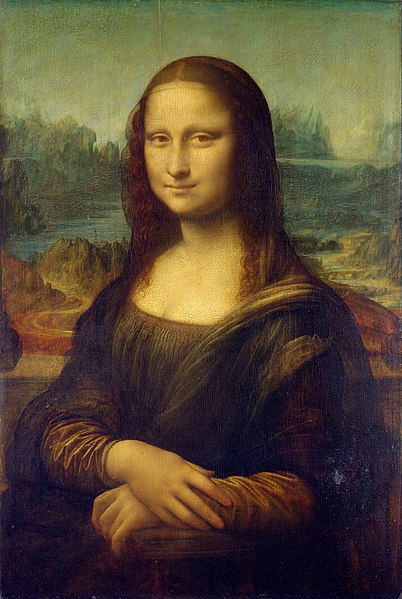
\includegraphics{monalisa}
			\caption[The Mona Lisa]{The Mona Lisa.\\
				\url{https://commons.wikimedia.org/wiki/File:Mona_Lisa,_by_Leonardo_da_Vinci,_from_C2RMF_retouched.jpg}}
			\labfig{marginmonalisa}
		\end{marginfigure}
	\item[Margin toc] Finally, since we have wide margins, why don't add 
		a little table of contents in them? See \verb|\margintoc| for 
		that.
	\item[Hyperref] \verb|hyperref| is loaded and by default we try to 
		add bookmarks in a sensible way; in particular, the bookmarks 
		levels are automatically reset at \verb|\appendix| and 
		\verb|\backmatter|.
\end{description}

\section{What this class does not}
\labsec{doesnot}

As anticipated, the styling is left to the user. Indeed, every book may 
have sidenotes, margin figures and so on, but each book will have its 
own fonts, toc style and so on. For this reason, we only provide 
sensible defaults. The github repository is organised as follows.

\begin{description}
	\item[kaobook.cls] The class file, which contains the definitions of 
		the commands and the environments and loads the required 
		packages.
	\item[packages.sty] Loads other packages to improve the experience 
		of the user (for instance, \verb|ams*| packages are loaded here 
		as they are not required in every book).
	\item[commands.sty] Complements to the packages, \eg the 
		specifications of the \verb|theorem| environments.
	\item[style.sty] Page layout, formatting of the titles\ldots
\end{description}

Moreover, there is a folder containing this very book as an example.
